\documentclass[a4paper,11pt]{kth-mag}
\usepackage[T1]{fontenc}
\usepackage{textcomp}
\usepackage{lmodern}
\usepackage{datetime}
\usepackage[utf8]{inputenc}
\usepackage[swedish,english]{babel}
\usepackage{modifications}
\usepackage{algorithm2e}
\usepackage{graphicx}
\usepackage{subcaption}
\usepackage{url}
\selectlanguage{swedish}
\title{Benchmarking Beginner Algorithms for
           Rubik's cube}

\author{Andreas Nilsson  anil9@kth.se\\Anton Spång  aspang@kth.se}
\date{\today}

\blurb{DD143X - Bachelor Thesis\\Supervisor: Michael Schliephake\\Examiner: Örjan Ekeberg}
\begin{document}
\frontmatter
\pagestyle{empty}
\removepagenumbers
\maketitle
\selectlanguage{english}
\begin{abstract}
 Over the years different algorithms have been developed to step-by-step solve parts of the Rubik's cube until finally reaching the unique solution. This thesis explores two commonly known beginner algorithms for solving Rubik’s cube to find how they differ in solving speed and amount of moves. The algorithms were implemented and run on a large amount of scrambled cubes to collect data. The results showed that Layer-by-layer with daisy algorithm had a lower average amount of moves than the Dedmore algorithm. The main difference in amount of moves lies in the steps that solve the last layer of the cube. The Layer-by-layer with daisy algorithm uses only one-seventh of the time-consuming operations that Dedmore algorithm uses, which concludes that it is more suitable for speedcubing. 


  


\end{abstract}
\clearpage
\begin{foreignabstract}{swedish}
  Över åren har ett antal olika algoritmer utvecklats för att steg-för-steg lösa delar av Rubik's kub för att till sist komma fram till den unika lösningen. Denna rapport utforskar två allmänt kända nybörjaralgoritmer för att lösa Rubik's kub, för att finna hur dem skiljer sig åt i tid samt antal operationer för att nå lösningen. Algoritmerna implementerades och kördes på ett stort antal blandade kuber för att samla data. Resultatet visar att Lager-för-lager med daisy algoritmen hade ett lägre genomsnittligt antal förflyttningar jämfört med Dedmore algoritmen. Den största skillnaden i antalet förflyttningar ligger i stegen som löser sista lagret av kuben. Lager-för-lager med daisy algoritmen använder bara en sjundedel av de mest tidskrävande förflyttningarna jämfört med Dedmore algoritmen, slutsatsen av detta är att Lager-för-lager med daisy algoritmen är bättre lämpad för lösning av kuben på tid.  
\end{foreignabstract}

\clearpage
\tableofcontents*
\mainmatter
\section{Terminology} 
	\begin{description}
		\item[Cubie] one of the twenty-six small cubes that make up the Rubik's cube.
		\item[Scramble] perfoming some amount of random operations on a solved cube to reach a non-solved state.
		\item[Layer] the nine cubies making up a side or the 8 cubies all around the cube either vertically or horizontally starting from a center-positioned cubie (middle layer).
		\item[Operation] rotating one layer of the cube.
	\end{description}

\pagestyle{newchap}
\chapter{Introduction}
\begin{figure}
	\centering
	\begin{subfigure}[b]{0.3\textwidth}
		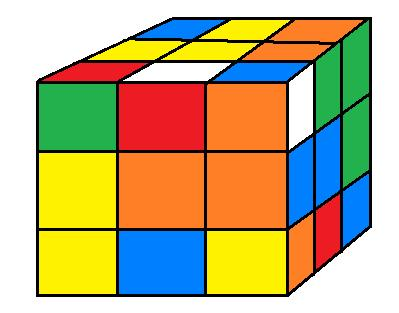
\includegraphics[width=\textwidth]{figs/scramble.jpg}
		\caption{Scrambled cube}
		\label{fig_1}
	\end{subfigure}
	\begin{subfigure}[b]{0.3\textwidth}
		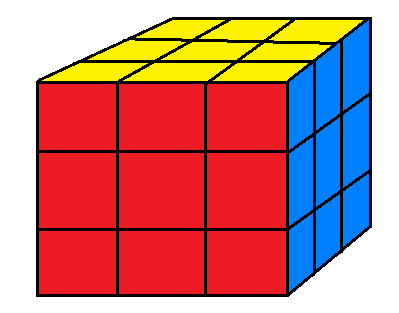
\includegraphics[width=\textwidth]{figs/DONE.png}
		\caption{Solved cube}
		\label{fig_2}
	\end{subfigure}
	\caption{}
\end{figure}

The Rubik’s cube is a 3-D combination puzzle, where each side of the cube is covered with nine squares in six possible colours: white, red, blue, orange, green and yellow. It was invented by the professor of architecture Ernő Rubik as a teaching tool to help his students to understand 3D objects. It was not until he scrambled his new cube and tried to restore it, that he realize his creation was a puzzle. Originally the Rubik's cube was called the Magic Cube and was licensed to be sold by the american toy company Ideal Toy Company in 1980. \cite{Rubiks}.\\\\
When solving the cube the idea is to start with a scrambled cube, meaning that the cubies are randomly positioned by executing random operations on the cube (fig \ref{fig_1}). The goal is to obtain the unique solution where each side of the cube is covered with only one colour per side (fig \ref{fig_2}). Different algorithms have been developed to solve subproblems one at the time with a series of operations to reach the unique solution. Many algorithms are based on the idea to solve it one layer at the time.\\\\
If you were to randomly rotate the faces in an attempt to solve the cube, there is almost zero chance of achieving the solved state in your lifetime, because of all the possible permutations of the cube. There are $4.3 * 10^{19}$ (or 43 quintillion) \cite{Faculty} different states. Assuming you get to a unique state every second it would take more than 130 billion years to test 10\% of the cubes possible states [Appendix A].\\\\
There are two major ways to compete in solving the Rubik’s cube: the least amount of moves and solving the cube as fast as possible (speedcubing).

\section{Problem}
This thesis will explore two commonly known beginner algorithms for human solving of Rubik’s cubes to find the differences. Both algorithms are based on the idea to solve the cube one layer at the time, which is the easiest way for the human mind to solve this kind of problem \cite{Lar5}. We will evaluate the algorithms operation variance and the number of operations to reach a solved state, to find the most move-efficient of them both.\\\\
The thesis will not include any empirical study of humans solving the cube with different beginner algorithms, and will instead rely on data gathered from computations.
The problem was stated as follows:
\begin{itemize}
\item[] Which of the beginner algorithms would be more effective for speedcubing?
\item[] Which of the beginner algorithms solves the cube with the least amount of moves?
\end{itemize}
\section{Purpose}
The purpose of testing the algorithms is to find out which uses the least amount of moves and to find out which algorithm suits speedcubing best by analyzing the usage of different operations. The reason the operations shows if the algorithm is suitable for speedcubing is because some of the operations are more time-consuming than others. The inexperienced user will find this as a guideline as to which algorithm to start his/her journey towards solving the Rubik’s cube.
\section{Structure}
The second section will introduce the reader to concepts necessary to understand the algorithms implemented and benchmarked. The third section will explain the Algorithms used in this thesis together with explanations of the representation and implementation of the cube. The fourth section will be presenting the results and the fifth section contains a discussion regarding the results. Following that is a conclusions section that completes the circle of the thesis, answering the problem statements. Lastly the references used to this thesis will be listed followed by appendix containing computations and data.  


\chapter{Background}
This section provides the reader with knowledge of: how the cube works, move operations, competitions and the algorithms that are in focus for this thesis.
\section{Rubik's Cube}
Explanation of how the cube is constructed and the different notations for the operations.
\paragraph{Description}
The cube consists of 26 cubies with three, two or one visible side depending on the type of cubie. There is one core piece consisting of three axes holding the center pieces together \cite{MadeHow}. 
  The corner and edge pieces (fig \ref{fig_3})  are the cubies that are movable to different edge and corner positions, the center pieces (fig \ref{fig_3}) can only be moved according to the axis.  
\paragraph{Operations}

An operation is a movement of a layer on the cube and is communicated by notations (abbreviations of operation name) in the Rubik's cube community. This thesis uses the notations used by the World Cube Association (WCA) \cite{WCA1} explained below:\\
Clockwise 90 degrees:\\
F - Front face\\
B - Back face\\
R - Right face\\
L - Left face\\
U - Upper face\\
D - Bottom face\\
The thesis also uses notations for turning the middle layer, defined as follows \cite{Ruwix}:\\
M - Middle layer vertical, in the same direction as L\\
E - Middle layer (Equatorial) horizontal, in the same direction as D\\
To denote the anti-clockwise 90 degrees rotation just put a single citation mark (‘) after the letter. For example F’ - move front face anti-clockwise 90 degrees.
To denote clockwise 180 degrees rotation just put (2) after the letters described above.\\\\


\begin{figure}[t]
	\centering
	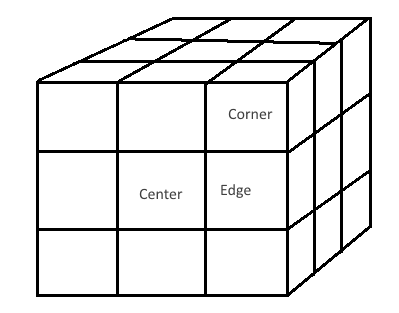
\includegraphics[width= 0.4\textwidth]{figs/representation.png}
	\caption{Cubie types}
	\label{fig_3}
\end{figure}
\section{Competitions}
There are two types of competitions for the cube that are relevant for this thesis.
\paragraph{Speedcubing}
When competing in an official event regulated by the WCA, the competitor has at maximum 15 seconds of inspection time of the cube before the solve begins \cite{WCA2}. The time stops when the competitor have reached the unique solution. 
\paragraph{Fewest moves}
The competitors have 60 minutes without any inspection time and the competitor should also be able to hand in a written solution with the notations used in the correct format \cite{WCA2}.
\section{Algorithms}
The physical methods for solving the cube by hand matches the mathematical definition of an algorithm. Unlike many of the “near-optimal solvers” (some of which simulates several moves ahead to find the optimal move \cite{Kociemba}), these algorithms can with little effort be taught to humans. The algorithms are built on many heuristics that guarantees a solution, but the number of moves exceeds the proven maximum amount to solve any cube in any state (20) \cite{cube20}. With the algorithms as heuristics comes multiple ways to solve each step.\\\\
The algorithms in focus in this thesis is based on solving the cube layer-by-layer. This means that the algorithms divides the cube into layers which makes it possible to solve the layers in steps/subproblems without breaking the layers previously completed.
\paragraph{Layer-by-layer using daisy algorithm}
\begin{figure}[b]
	\centering
	\begin{subfigure}[!b]{0.3\textwidth}
		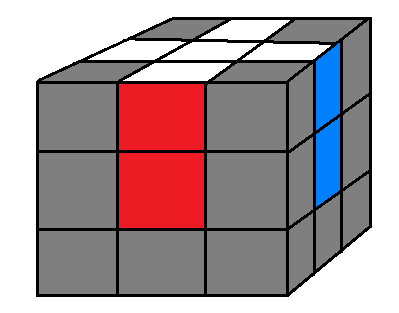
\includegraphics[width=\textwidth]{figs/step1.png}
		\caption{The white cross done}
		\label{fig_4}
	\end{subfigure}
	\begin{subfigure}[!b]{0.3\textwidth}
		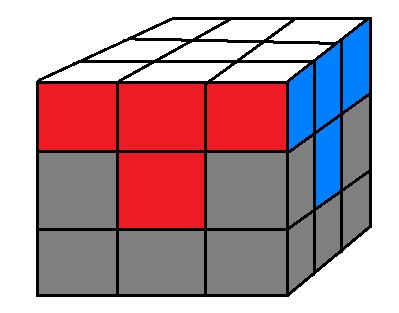
\includegraphics[width=\textwidth]{figs/step2.png}
		\caption{First layer complete}
		\label{fig_5}
	\end{subfigure}
	\caption{}
\end{figure}
Due to this algorithm has no name, it will from here be referred to as Layer-by-layer with daisy (or Lbl with daisy for short). The daisy-part of the name refers to the algorithm to solve the white cross by first make a cross with white edges and a yellow center and then turn the white edges over to the opposite side, completing the white cross in the bottom \cite{Shellie}.
\subsubsection{1. White cross}
The goal here is to achieve a white cross, so that the white center-piece is aligned with its 4 white edge-pieces in the bottom. For it to be a completed step, the second color of the white edge-pieces must also align with it’s center-piece counterpart as shown in fig \ref{fig_4}.This is done using daisy's method, flipping the edges one at the time to make sure the edge-pieces on the vertical sides are aligned with the center-pieces on the same sides.
\subsubsection{2. White corners}
With the white cross done the next step is to complete the first layer by positioning the white corner-pieces correct between the cross edges (fig \ref{fig_5}). This is achieved with three different operation-combinations depending on the colour positions, all focusing on the upper-front-left corner of the cube.
\subsubsection{3. Middle layer edges}
The next step is to solve the middle layer by moving down a cubie from the middle of the third layer to the correct position on the second layer (fig \ref{fig_6}). 
\subsubsection{4. Yellow cross}
With the second layer complete (fig \ref{fig_7}) it is time to work on the yellow cross. This is achieved by applying one of two operation-combinations or both depending on how many white pieces that are correct positioned (fig \ref{fig_8}).  
\subsubsection{5. Yellow corners}
Positioning the yellow corners by applying different operations to move the edges depending och how many corners that are in position already. 
\subsubsection{6. Last layer permutation}
Now when the corners of the last layer are in position so that the top is all yellow, the only thing left to do is to positioning the pieces of the last layer so they match with the colours of the vertical sides. This is achieved by applying three different operation-combinations depending on if its edges or corners that should switch places. 
\begin{figure}[h]
	\centering
	\begin{subfigure}[!b]{0.3\textwidth}
		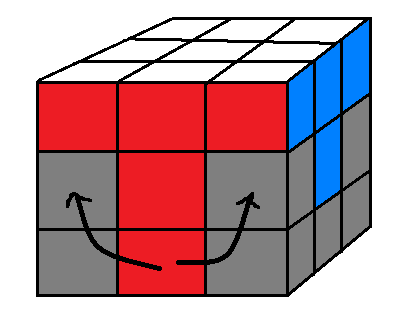
\includegraphics[width=\textwidth]{figs/step32.png}
		\caption{Technique for each side}
		\label{fig_6}
	\end{subfigure}
	\begin{subfigure}[!b]{0.3\textwidth}
		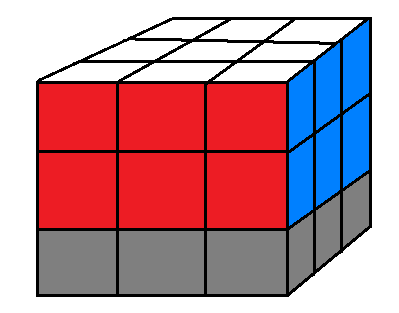
\includegraphics[width=\textwidth]{figs/step31.png}
		\caption{Middle layer complete}
		\label{fig_7}
	\end{subfigure}\caption{}
\end{figure}
\begin{figure}[h]
	\centering
	\begin{subfigure}[!b]{0.3\textwidth}
		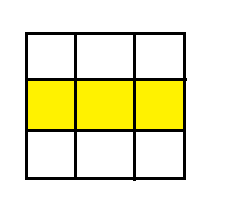
\includegraphics[width=\textwidth]{figs/step41.png}
	\end{subfigure}
	\begin{subfigure}[!b]{0.3\textwidth}
		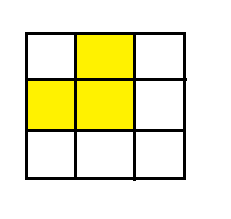
\includegraphics[width=\textwidth]{figs/step42.png}
	\end{subfigure}
	\begin{subfigure}[!b]{0.3\textwidth}
		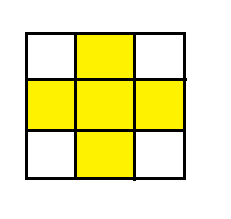
\includegraphics[width=\textwidth]{figs/step43.png}
	\end{subfigure}
	\caption{Different states to achieve the yellow cross}
	\label{fig_8}
\end{figure}
\newpage
\paragraph{Dedmore algorithm}
The dedmore algorithm differs from Lbl with daisy in focusing on a corners-first solution \cite{Dedmore}. It was one of the first solution guides to the Rubik's cube \cite{Ijsat}. The following steps can be found in more detail at the website created by Denny Dedmore himself \cite{Dedmore}.\\
\begin{figure}[b]
	\centering
	\begin{subfigure}[!b]{0.3\textwidth}
		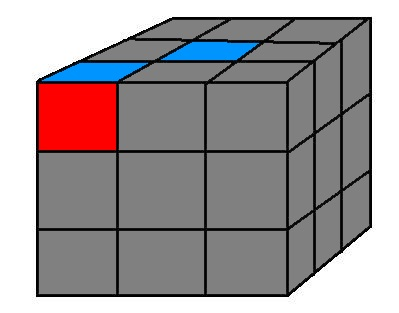
\includegraphics[width=\textwidth]{figs/rubiks-frst-corner.jpg}
		\caption{First corner in position}
		\label{fig_9}
	\end{subfigure}
	\begin{subfigure}[!b]{0.3\textwidth}
		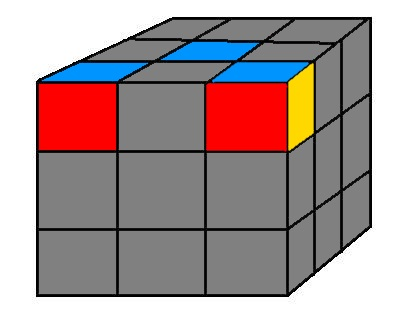
\includegraphics[width=\textwidth]{figs/rubiks-scnd-corner.jpg}
		\caption{Second corner in position}
		\label{fig_10}
	\end{subfigure}
	\begin{subfigure}[!b]{0.3\textwidth}
		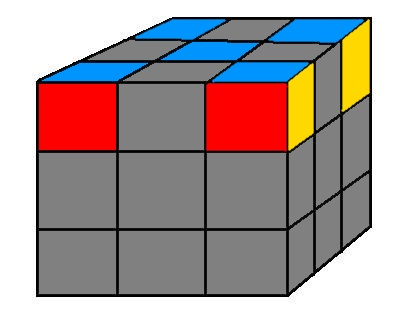
\includegraphics[width=\textwidth]{figs/rubiks-4-corners.jpg}
		\caption{Top edges in position}
		\label{fig_11}
	\end{subfigure}
	\caption{}
\end{figure}

\subsubsection{1. Top corners (the X)}
Start off by finding a starting corner. For example aim to solve the blue top face first. Rotate the cube to obtain the blue side of the corner in top position. Then move the blue center-piece into position without moving the corner. When this is done, rotate the whole cube to put the corner in the top left on the front side, as in the fig \ref{fig_9}.\\\\
Search for the next corner that should be positioned in the top right front side. Match the position of this corner to one of 6 scenarios and execute different operation-combinations to get it in position like the fig \ref{fig_10}. Rotate the cube and continue with the next corner. The goal of this step is to form a ‘X’ on the top face as in fig \ref{fig_11}.
\subsubsection{2. Top edges}
The goal of this step is to get the edges in place. The strategy is to get them in place one by one, by matching the cube to one of five scenarios and then execute an operation-combination for solving that scenario. When this step is finished the cube looks like fig \ref{fig_12}.
\subsubsection{3. Middle layer}
The next step is to solve the middle layer by moving down a cubie from the middle of the third layer to the correct position on the second layer (fig \ref{fig_6}). 
\subsubsection{4. Bottom corners}
Here the cube is turned upside down and the goal is again to build a (green) `X' with the corners(fig \ref{fig_13}). This is done by regarding the 4 corner cubies as 2 pairs and moving each pair into correct position. The correct pair can be either in each other's position, or diagonally from each other. Both requiring different operation-combinations to solve.\\\\When the corner pairs are in position, the next part is to make sure the cubies are facing the correct way. This is done by matching the cube to one of seven different scenarios, and perform an operation-combination. This might have to be repeated up to 3 times for the step to be completed. 
\subsubsection{5. Bottom edges}
In this step, at least one edge is already in the correct place (the color might be switched as in fig \ref{fig_14}). Find that edge and put it on the front side. Then position every other edge correctly by executing an operation-combination up to 2 times.\\\\
When every edge are correctly positioned, there are 2 possible states left. Each requires a different sequence of operations to solve. The ‘fish’ pattern (fig \ref{fig_15}) and the ‘H’ pattern (fig \ref{fig_16}). Execute the sequence for the pattern and the cube is solved.
\begin{figure}[bh]
	\centering
	\begin{subfigure}[!b]{0.3\textwidth}
		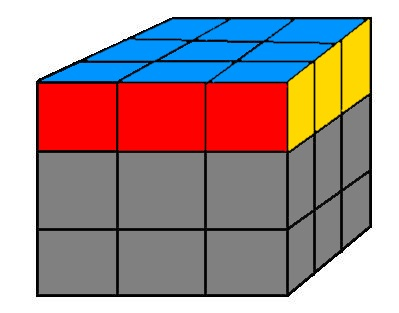
\includegraphics[width=\textwidth]{figs/rubiks-top-edges.jpg}
		\caption{Top edges in position}
		\label{fig_12}
	\end{subfigure}
	\begin{subfigure}[!b]{0.3\textwidth}
		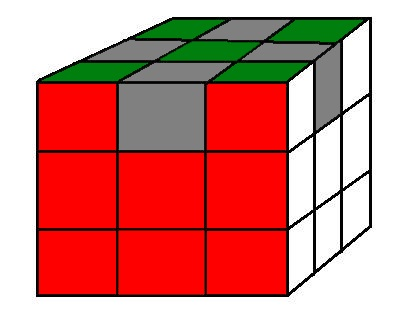
\includegraphics[width=\textwidth]{figs/rubiks-bottom-edges.jpg}
		\caption{The green X}
		\label{fig_13}
	\end{subfigure}
	\begin{subfigure}[!b]{0.3\textwidth}
		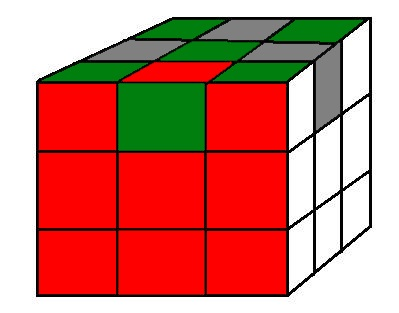
\includegraphics[width=\textwidth]{figs/last-edge-correct.jpg}
		\caption{One edge correctly placed}
		\label{fig_14}
	\end{subfigure}
	\caption{}
\end{figure}
\begin{figure}[bh]
	\centering
	\begin{subfigure}[!b]{0.3\textwidth}
		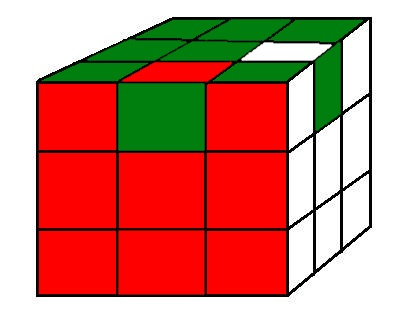
\includegraphics[width=\textwidth]{figs/fish-pattern.jpg}
		\caption{Fish pattern}
		\label{fig_15}
	\end{subfigure}
	\begin{subfigure}[!b]{0.3\textwidth}
		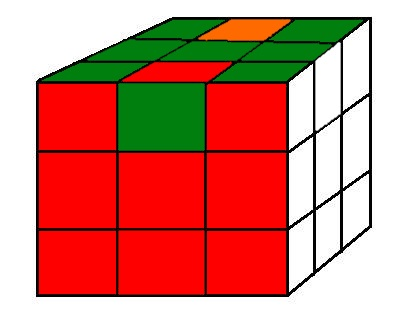
\includegraphics[width=\textwidth]{figs/H-pattern.jpg}
		\caption{H pattern}
		\label{fig_16}
	\end{subfigure}
	\caption{}
\end{figure}

\chapter{Method}
For this thesis the two methods used were implementation of algorithms and analysis of the data representation. An implementation was motivated considering that implementations allowed analysis and collection of data from multiple algorithm runs.
Both of the algorithms was implemented in Java and with the same built-in functions and data structures to rule out differences and obtain a realistic comparison.
The algorithms were run a number of times on different cubes to obtain a good set of data for the comparison. The data was obtained during the runs by gathering information such as: number of moves used, statistics of which moves used and number of times one algorithm used less moves than the other.  
For each algorithm the test data was evaluated by use of different operations, number of operations used and time-consuming operations.


\section{Cube representation}
 The cube was represented as six separate sides with nine positions per side, each of which has a color (see fig \ref{fig_17}). There exists no relation between positions in different sides; unlike the physical cube, where for example an edge has two colors. This means any correctly performed operation needed to move the colours to the correct side and location. The only way to keep the rules of the physical cube (correct colour-combination of a cubie) were to enforce them during the operations.\\\\
 For example performing the `F' operation (flip the front layer 90 degrees clockwise) on the cube shown in fig \ref{fig_17} would result in these internal assignments:
 \begin{verbatim}
		Side tempTop = new Side(top);
		Side tempFront = new Side(front);
		top.c7 = left.c9;
		top.c8 = left.c6;
		top.c9 = left.c3;
		left.c3 = bot.c1;
		left.c6 = bot.c2;
		left.c9 = bot.c3;
		bot.c1 = right.c7;
		bot.c2 = right.c4;
		bot.c3 = right.c1;
		right.c1 = tempTop.c7;
		right.c4 = tempTop.c8;
		right.c7 = tempTop.c9;
		front.c1 = tempFront.c7;
		front.c2 = tempFront.c4;
		front.c3 = tempFront.c1;
		front.c4 = tempFront.c8;
		front.c6 = tempFront.c2;
		front.c7 = tempFront.c9;
		front.c8 = tempFront.c6;
		front.c9 = tempFront.c3;
\end{verbatim}
\paragraph{Time-consuming operations}
The authors own experience (as novices) of the operations indicates that the operations E and M are most time-consuming because they both work with the middle-layer (vertically and horizontally).
Due to the fact that no empirical studies were conducted, an assumption was made that operations working with the middle layer took a beginner twice as long as `normal' operations to perform.

\begin{figure}[b]
	\centering
	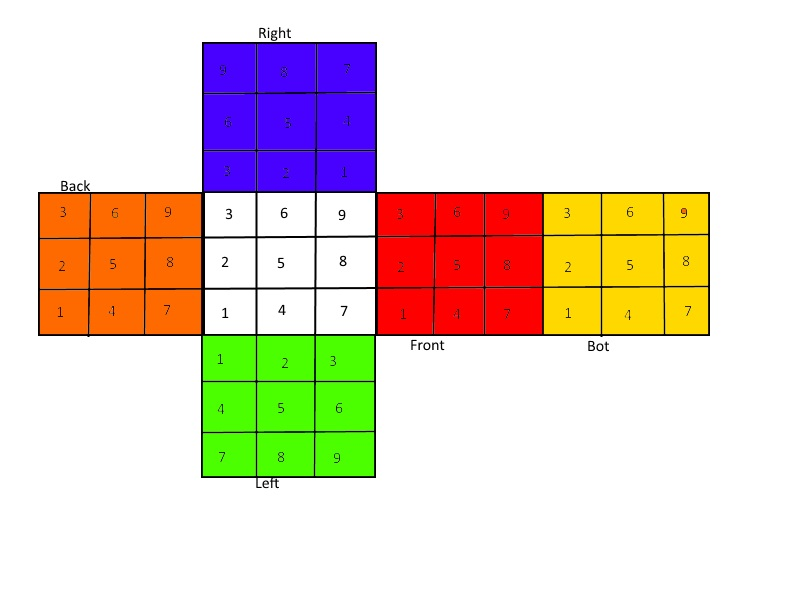
\includegraphics[width= 0.8\textwidth]{figs/cubeorder.jpg}
	\caption{Side numberings}
	\label{fig_17}
\end{figure}  
\section{Scramble}
The idea of the scrambler is to always start with a solved cube. The scramble is simulated by making a large amount of operations in pseudo-random sequence [Algorithm 1]. The scrambled cube is saved to a list awaiting the two solvers to pick and solve it.\\\\
\RestyleAlgo{boxed}
	\begin{algorithm}[H]
	\caption{Scramble}
	\KwIn{A cube, Number of operations to be made}
	\KwOut{A scrambled cube}
	Let rand be a psuedo-random generator.\\
	\For{Number of op to be made}{int opNr = rand.nextInt(Tot num of op)\\ \Switch{opNr}{ All operations represented by a number, perform the operation with the number opNr}}

	\end{algorithm}

\section{Implementation}
	Both algorithms contains several steps and all of them uses the same structure. Starting off by looking if the goal of the step is already achieved. While the goal is not achieved: put the cube in a (by the algorithm) desired position and then perform operations in an order given by the algorithm to reach the solution state for the step [Algorithm 2].
	\raggedbottom
	\paragraph{Complexity} The steps of both algorithms used the same general idea with the same data-structures in the implementation (see [Algorithm 2]). Using the same data-structure simplifies the comparison of the algorithms due to no big differences in implementations. Both algorithms run in linear time: the loops that break when a step is complete have a constant maximum number of iterations, because each step will focus on a finite part of the cube in form of a layer, resulting in a finite amount of permutations to try.
	\RestyleAlgo{boxed}
	\begin{algorithm}[H]
	\caption{The general idea of algorithm steps}
	\KwIn{A cube}
	\KwOut{A cube that has a step solved}
		\If{stepIsDone(cube)}{return cube}
		\While{not(stepIsDone(cube))}{\If{readyForOperations(cube)}{Perform the operations necessary to complete the step}\Else{\While{not(readyForOperations(cube))}{Operations to get the cube in a state to be able to perform the steps operations}}}
	\end{algorithm}

	
\chapter{Results}

In this section the results are displayed as a comparison of the algorithms amount of moves used, statistics for specific operation usage and number of times the algorithm used least amount of moves. The amount of moves in each step of both algorithms are also presented.\\\\ 
Fig \ref{fig_18} represents the sum of executions that used the same amount of moves, where the x-axis is amount of moves and the y-axis number of runs.
As shown by the highest pillars for both algorithms, the Lbl with daisy algorithm had a lower average (170) amount of moves than the dedmore algorithm (189). Turning the whole cube in any direction was not counted for as a move.\\\\
Fig \ref{fig_19} represents a comparison of the number of runs the algorithms used least amount of moves, with the y-axis as number of runs. 
This shows that over ten thousand scrambled cubes the Lbl with daisy algorithm won 71\% of the time, they got equal amount of moves 1\% of the time and dedmore algorithm had the fewest in comparison 28\% of the time.\\\\
Fig \ref{fig_20} represents the average use of operations for both algorithms over all runs with the x-axis as the average number of times the operations where used. \\The data for both fig \ref{fig_19} and fig \ref{fig_20} can be found in detail in Appendix B.\\\\ 
Fig \ref{fig_21} and fig \ref{fig_22} represents the amount of moves used in each step for both algorithms. By comparing fig \ref{fig_21} and \ref{fig_22} it is clear that the biggest difference in amount of moves are between the middle layer step and the last steps of the two algorithms.\\\\
Fig \ref{fig_23} visualizes the average total time to solve the cubes and how much of the time that was spent on time-consuming operations (included in total time). 
\begin{figure}[h!]
	\centering
	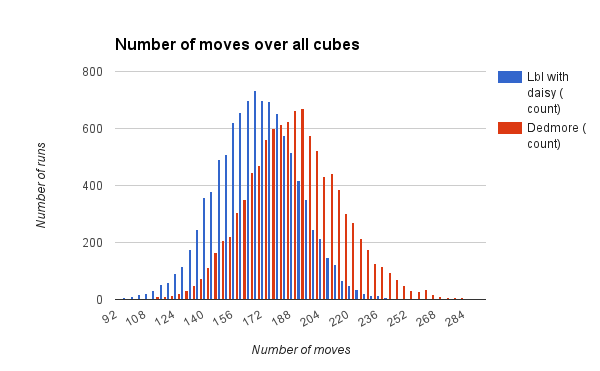
\includegraphics[width= 1.1\textwidth]{figs/graphone.png}
	\caption{}
	\label{fig_18}
\end{figure}
\begin{figure}[ht!]
	\centering
	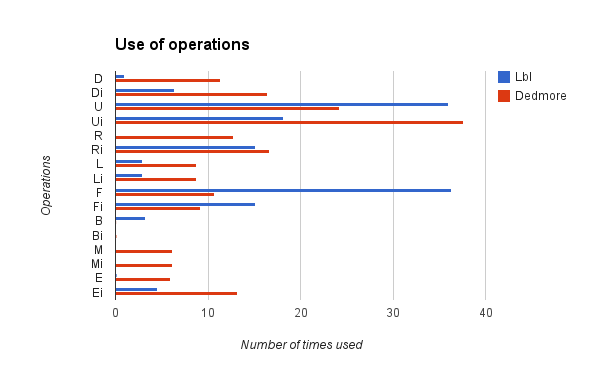
\includegraphics[width= 1.0\textwidth]{figs/graphtwo.png}
	\caption{}
	\label{fig_19}
\end{figure}
\begin{figure}[ht!]
	\centering
	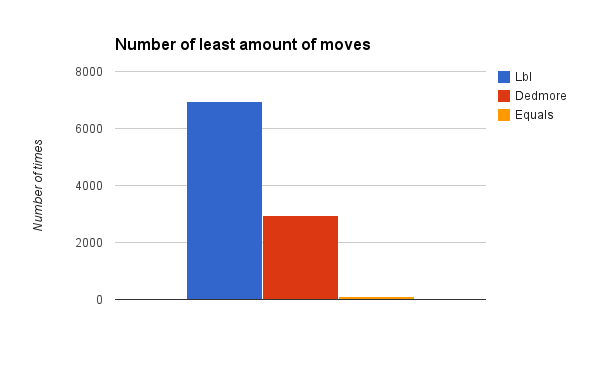
\includegraphics[width= 1.0\textwidth]{figs/graphthree.png}
	\caption{Average use of operations}
	\label{fig_20}
\end{figure}
\begin{figure}[ht!]
	\centering
	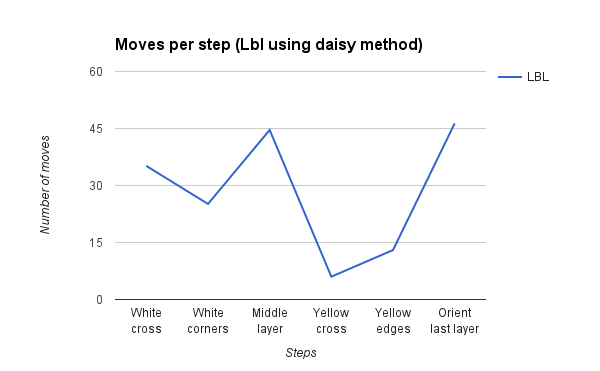
\includegraphics[width= 1.0\textwidth]{figs/lbldaisysteps.png}
	\caption{Number of moves per step}
	\label{fig_21}
\end{figure}
\begin{figure}[ht!]
	\centering
	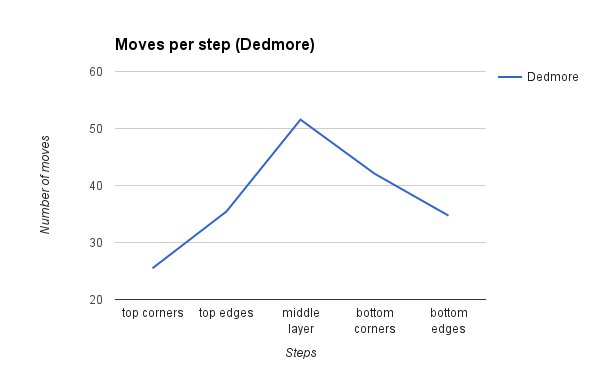
\includegraphics[width= 1.0\textwidth]{figs/dedmoresteps.png}
	\caption{Number of moves per step}
	\label{fig_22}
\end{figure}
\begin{figure}[ht!]
	\centering
	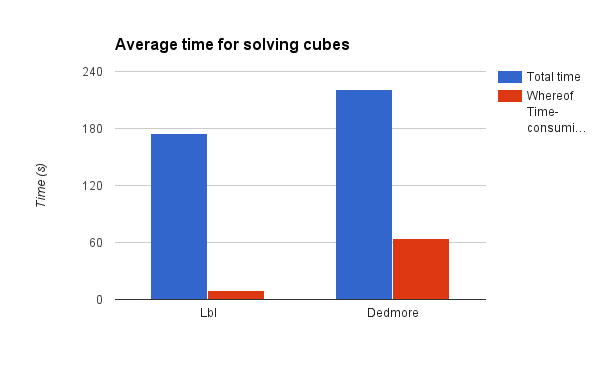
\includegraphics[width= 1.0\textwidth]{figs/time.png}
	\caption{Time-consuming operations and total time}
	\label{fig_23}
\end{figure}
\chapter{Discussion}
In this section we discuss the results in form of comparisons and reflect on why these results where given. We also discuss any errors that could have had an impact on the final results.
\section{Comparison}
As we can see in the results fig \ref{fig_18}, Lbl with daisy algorithm has the lowest amount of moves the majority of the times. Lbl with daisy algorithm also has the lowest minimum and maximum amount of moves with 95 and 253 respectively. The corresponding values for the Dedmore algorithm are 96 and 292 as can be seen in fig \ref{fig_18} and in Appendix B. This shows that Lbl wins in lowest average, best case and worst case and the result of this is shown in fig \ref{fig_19}.\\\\
The algorithms often assumed the correct cubies to be on a certain side of the cube, in reality this simply means rotating the cube to a desired position. The implemented versions prioritized execution of operations instead, to get the cube into position, which led to an increase in the amount of total operations. This might explain the frequent uses of a few operations, for example U, Ui and F, shown in fig \ref{fig_20}.\\\\
According to the result graphs fig \ref{fig_21} and fig \ref{fig_22} the part of the algorithms with the biggest differences in amount of moves are the steps solving the middle layer and last layer. But with the middle layer using the same technique in both algorithms the focus is turned to the last layer steps, to find differences affecting the number of moves. The steps in focus are yellow cross (average 6 moves) and yellow corners (average 13 moves) in Lbl with daisy algorithm and bottom corners (average 42 moves) in Dedmore algorithm. The cube has two layers completely solved before these steps are performed. These steps are comparable because they are solving the same layer of the cube, which limits the choice of operation-combinations to use without destroying parts of the first two layer that are completed.\\\\ 
The reason why the two steps in Lbl with daisy (total average 19 moves) uses less moves than dedmores step are because of the difference in strategy in the steps and a possible error described below.
The step Yellow cross has three possible starting positions, which needs two different operation-combinations or both of them combined, and each operation-combination consists of 6 moves.
The step Yellow corners has the same structure as yellow cross with three cases. Two of these cases are operation-combinations needed to be able to perform the solving case depending on the permutation of the cube. Each case uses at a minimum 8 moves, the solving case can use 16 moves in the worst scenario.\\\\
Analyzing Dedmores bottom corner step shows that it works with two corners at the time, positioning them by using two cases of operation-combination for the first pair (11 moves each) and one case if needed for the second pair (11 moves). Now in the finishing part of the step the cube can be matched with one of seven possible states and when matched an operation-combination (10 moves) needs to be performed to solve the step. That operation-combination should (according to the description of the step) be performed at a maximum of three times before the step is finished, which turned out to be incorrect. We have found that it is possible that the finishing part of the step needs more than three performed operation-combinations, making the amount of moves go up over 30 in worst case with a top, for just this part. According to the description of the step the max amount of moves should be 52 and least amount of moves should be 21, making the least amount of moves for Dedmore's bottom corner step higher than the average for Lbl with daisys steps.\\\\   
The data in fig \ref{fig_20} and Appendix B shows that Dedmore used both E, Ei and M, Mi more than Lbl with daisy. With this results in mind we investigate the graph \ref{fig_23} which shows the amount of time-units used by the time-consuming operations compared to the total time. This should, according to the assumptions made, imply that Dedmore uses more time than Lbl with daisy algorithm because of the time-consuming operations used.   		     


\section{Errors}
Converting the algorithms effeciently from description of physical solving of the cube to the code solver proved to be challenging. Ambigous and unfinished description of steps in the algorithms led to an extra amount of operations on the cubes. This had an impact on the final result.

      

\chapter{Conclusion}
The measurements shows that the Layer-by-layer using daisy algorithm solved the cube with the least amount of moves in more than 70\% of the 10,000 executions made. It also shows that the same algorithm had the lowest moves in minima and maxima on the tested cubes. This concludes that the Layer-by-layer using daisy algorithm is the better choice of algorithm regarding the least amount of moves.\\\\
Time measurements shows that Layer-by-layer using daisy algorithm is more suitable for speedcubing than Dedmore. This conclusion is based on the statistics of operation-usage, showing that Dedmore used these time-consuming operations seven times more frequently than Lbl with daisy algorithm.
This is also supported by the assumption made on the time-differences between time-consuming and normal operations.


\renewcommand{\bibname}{References}
\bibliographystyle{plain}
\bibliography{references}

\appendix
\addappheadtotoc
\chapter{Calculation of randomly rotated faces}\label{appA}
Assumption: Every second you get to a new state.\\
There are $4.3*10^{19}$  different states (rounded down) \cite{Faculty}.
10\% of the different states:\\
$4.3*10^{19}*0.1=4.3*10^{18}$ \\
$4.3*10^{18}$ seconds to years = $136.4*10^{9}$ years.

\label{App:AppendixB}
\chapter{Data}
	
		Average use of operations.\\
		\begin{tabular}{|l|l|l|}
		\hline
		Operations & Lbl & Dedmore \\ \hline
		D & 1.0479 & 11.4515 \\ \hline
		E & 0.1197 & 6.0673 \\ \hline
		F & 36.4233 & 10.7832 \\ \hline
		B & 3.1820 & 0.0648 \\ \hline
		Ri & 15.0851 & 16.8868 \\ \hline
		L & 2.9329 & 8.7679 \\ \hline
		M & 0.000 &	6.1943 \\ \hline
		Ui & 18.1466 & 37.7807 \\ \hline
		U & 36.0456 & 24.2579 \\ \hline
		Bi & 3.1820 & 0.1031 \\ \hline
		Mi & 0.000 & 6.1943 \\ \hline
		Li & 2.9329 & 8.7187 \\ \hline
		R & 25.0051 & 12.7996 \\ \hline
		Ei & 4.5945 & 13.3863 \\ \hline
		Fi & 15.1346 & 9.2321 \\ \hline
		Di & 6.4249 & 16.5976 \\ \hline
		\end{tabular}
		\\\\
		Number of times the algorithms had least amount of moves.\\
		\begin{tabular}{|l|l|l|}
		\hline
		Lbl & Dedmore & Equals \\ \hline
		7098 & 2819 & 83 \\ \hline
		\end{tabular}
		\\\\
		Min and max moves \\
		\begin{tabular}{|l|l|l|}
		\hline
		 & Lbl with daisy algorithm & Dedmore \\ \hline
		Average amount of moves & 170 & 189 \\ \hline 
		Min amount of moves & 95 & 96 \\ \hline
		Max amount of moves & 253 & 292 \\ \hline
		\end{tabular}		

	
\end{document}
